\documentclass[10pt,a4paper]{article}
\usepackage[utf8]{inputenc}
\usepackage[T1]{fontenc}
\usepackage[margin=1.8cm,top=2.6cm,bottom=2.2cm]{geometry}
\usepackage{parskip}
\usepackage{microtype}
\usepackage{amsmath,amssymb,mathtools}
\usepackage{array,booktabs,tabularx}
\usepackage[table]{xcolor}
\usepackage{graphicx,float}
\usepackage{titlesec}
\usepackage{enumitem}
\usepackage{fancyhdr}
\usepackage{tcolorbox}
\usepackage[colorlinks=true,linkcolor=black,citecolor=black,urlcolor=blue!55!black,breaklinks=true]{hyperref}
\urlstyle{same}

\graphicspath{{../figures/}}

\renewcommand\thesection{\Roman{section}}
\numberwithin{equation}{section}

\titleformat{\section}{\large\bfseries}{\thesection.\;}{0em}{}[\titlerule]
\titleformat{\subsection}{\normalsize\bfseries}{}{0em}{}
\titlespacing{\section}{0pt}{1.6ex plus .2ex}{0.6ex}
\titlespacing{\subsection}{0pt}{1.0ex}{0.3ex}

\pagestyle{fancy}
\fancyhf{}
\setlength{\headheight}{15pt}
\fancyhead[L]{\small\textit{SWV Forward Model}}
\fancyhead[R]{\small Aaran Nihalani $\bullet$ Eton iGEM Dry Lab}
\fancyfoot[C]{\small\thepage}
\renewcommand{\headrulewidth}{0.35pt}

% ---- macros -----------------------------------------------------------
\newcommand{\cit}[1]{[#1]}
\newcommand{\R}{\mathbb{R}}
\newcommand{\bm}[1]{\boldsymbol{#1}}
\newcommand{\kcat}{k_{\mathrm{cat}}}
\newcommand{\Km}{K_m}
\newcommand{\nm}{\,\mathrm{nm}}
\newcommand{\dpeg}{d_{\mathrm{PEG}}}
\newcommand{\Gtot}{\Gamma_{\mathrm{tot}}}
\newcommand{\Gred}{\Gamma_{\mathrm{red}}}
\newcommand{\Gox}{\Gamma_{\mathrm{ox}}}
\newcommand{\Geq}{\Gamma_{\mathrm{eq}}}
\newcommand{\kref}{k_{\mathrm{ref}}}
\newcommand{\keff}{k_{\mathrm{eff}}}
\newcommand{\MMP}{[\text{MMP-9}]}
\newcommand{\avg}[1]{\left\langle #1\right\rangle}
\newenvironment{assump}{\small}{\smallskip}


\begin{document}

\begin{center}
{\LARGE\bfseries SWV Forward Model}\\[0.25em]
{\small\color{gray}Eton iGEM 2026, Dry Lab}
\end{center}
\vspace{0.4em}\hrule\vspace{0.7em}

%=======================================================================
\section{Overview}
\label{sec:overview}

Our sensor measures MMP-9, an enzyme found at much higher levels in chronic wounds (around 30 nM) than healing wounds (around 6 nM)~\cit{1}. The sensor is a small gold electrode coated with peptide probes that MMP-9 recognises and cuts. Each probe carries a methylene blue (MB) label, which exchanges electrons with the electrode to produce a current. When MMP-9 cuts a probe, that probe's label can no longer exchange electrons, so the overall current drops. We can measure the remaining current with square-wave voltammetry (SWV), which gives a single peak whose height reflects how many labels are still attached.

Our model predicts this peak for any MMP-9 concentration and incubation time, building it up in six connected steps. It starts by working out how many probes sit on the electrode surface and where each MB label sits relative to the gold. It then calculates the signal produced by a single probe and adds up every probe to give the signal from the whole electrode. Finally, it shows how to use the change in peak height from the SWV to find the fraction of probes cut, and calculates how fast MMP-9 cuts them. This links the MMP-9 level in the wound to the signal we measure.

The model shows that the peak height is exactly proportional to the number of intact probes. Scanning each electrode before and after incubation therefore gives the fraction of probes cut, $F_k$:
\begin{equation}
F_k = 1 - \frac{\Delta I(T)}{\Delta I(0)}
\label{eq:fk_headline}
\end{equation}
where $\Delta I(0)$ and $\Delta I(T)$ are the peak heights before and after incubation. After 30 minutes, the model predicts that MMP-9 in a healing wound cuts about 14\% of the probes, while in a chronic wound, MMP-9 cuts around 52\%. This is a large enough difference for the sensor to tell the two apart.

%=======================================================================
\section{The Electrode Surface}
\label{sec:surface}

We first need to know how many probes are on the gold and how far apart they are from one another. The number of probes per unit area is the \emph{coverage}, $\Gtot = 3\times10^{-12}\,\mathrm{mol\,cm^{-2}}$~\cit{2}.

\subsection{Probes per electrode}
Multiplying the coverage by Avogadro's number $N_A$ and the electrode area, $A = 0.017\,\mathrm{cm^2}$ (our device), gives the number of probes:
\begin{equation}
N = \Gtot N_A A = (3\times10^{-12})\cdot(6.02\times10^{23})\cdot(0.017) = 3.1\times10^{10}.
\label{eq:n_probes}
\end{equation}

\subsection{Spacing between probes}
Each probe has an area $a$ on average, where the area is equal to the reciprocal of the number of probes per unit area:
\begin{equation}
a = \frac{1}{\Gtot N_A} = 55\,\mathrm{nm^2} \quad (\text{using } 1\,\mathrm{cm^2} = 10^{14}\,\mathrm{nm^2}).
\label{eq:probe_area}
\end{equation}
We model the probes as being on a square grid, therefore the distance separating each probe, $s$, would be the square root of this area:
\begin{equation}
s = \sqrt{a} = 7.4\nm.
\label{eq:probe_spacing}
\end{equation}

\begin{figure}[H]
\centering
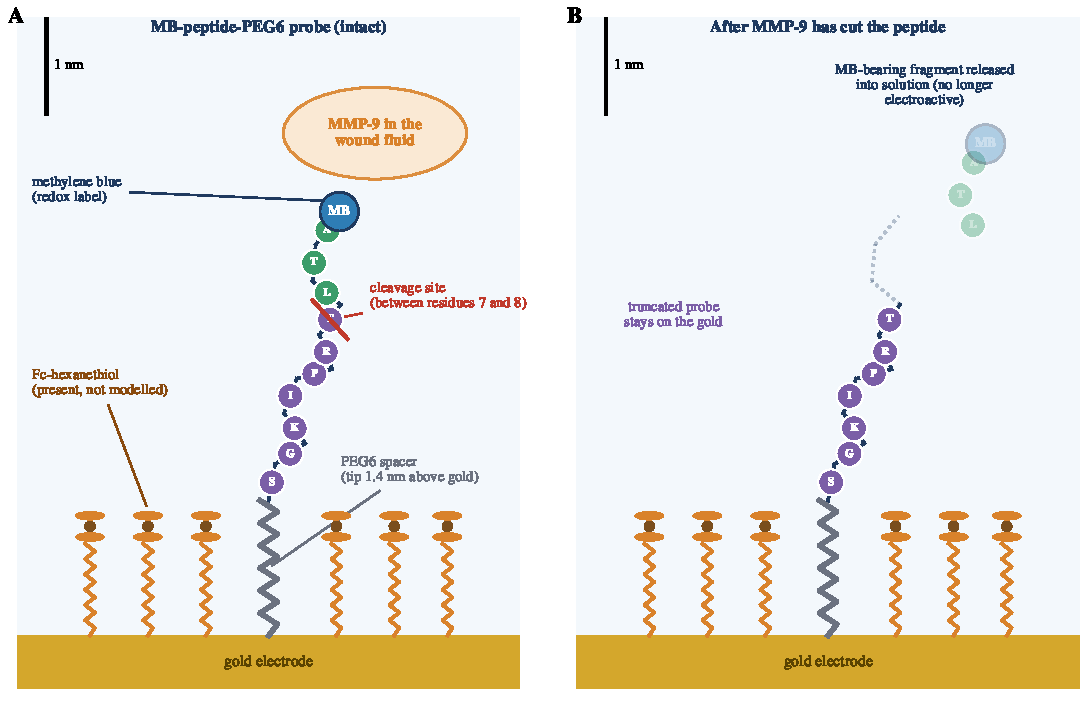
\includegraphics[width=0.78\textwidth]{swvr_01_assembly.pdf}
\caption{The electrode surface, drawn to scale. \textbf{A:} an intact probe: the peptide (SGKIPRTLTA) rises from the electrode on a PEG6 spacer and carries MB at its tip. The shorter ferrocene-hexanethiol (Fc-hexanethiol) fills the space between the probes. \textbf{B:} MMP-9 cuts the peptide at the red mark in A. The MB label is released and no longer contributes to the current.}
\label{fig:probe}
\end{figure}

\subsection{Ensuring the probes are independent}
In Section~\ref{sec:label}, we find that the MB label can move about $1.4\nm$ sideways from its anchor. Two labels can only hit each other if their anchors are closer than $2\times1.4 = 2.8\nm$. We have just calculated that the probes are $7.4\nm$ apart, so they will not interact with one another. This allows us to work out the signal from one probe and then multiply by the number of probes to get the total signal.

Every single probe on the electrode is around $7.4\nm$ from its neighbours, far enough apart that each one behaves independently.

%=======================================================================
\section{Where the MB Label Sits}
\label{sec:label}

The current depends on how far the MB label is from the gold, because electrons have to cross this distance to reach it. The further away the label is, the slower it exchanges electrons, so a small change in distance can have a large effect on the signal. The probe has two parts: a PEG6 spacer attached to the gold, and the peptide on top of it, with MB at its tip. The peptide is not rigid; it constantly moves and bends, so each MB label sits at a slightly different height. We therefore want to find how tall the spacer is, and the range of distances at which the MB label can sit above it.

\subsection{Modelling the peptide}
The peptide is flexible, so we can model it as a chain of short, stiff segments joined by free hinges, each pointing in a random direction. This is known as a freely jointed chain. Over very short distances the peptide is fairly rigid, so it will keep pointing in the same general direction, but over longer distances its small bends add up until it could be pointing in any direction. The length at which this happens is called the Kuhn length, $b = 0.76\nm$, which is about the length of two amino acids~\cit{3}. Our peptide has 10 amino acids, each $0.38\nm$ long so we can model it as
\begin{equation}
N_K = \frac{10\times0.38}{0.76} = 5 \text{ independent segments.}
\label{eq:nkuhn}
\end{equation}

\subsection{One segment}
We first need to find how much height a single segment adds to the label on average. A segment of length $b$, tilted at an angle $\theta$ from the vertical, adds height $X = b\cos\theta$. Since the segment points in a random direction, it is equally likely to move the label up or down, so on average it adds no height. However, an average of zero doesn't mean the segment has no effect, only that up and down are equally likely. To measure how far it typically moves the label, we square the heights and take the average, giving us
\begin{equation}
\avg{X^2} = \frac{b^2}{3}.
\label{eq:x2}
\end{equation}

\begin{itemize}
  \item A segment of length $b$ tilted at an angle $\theta$ from vertical adds height $X = b\cos\theta$. This is positive if the segment points upwards and negative if it points downwards.
  \item Because the segment points in a random direction, $u = \cos\theta$ is equally likely to take any value from $-1$ to $1$.
  \item To find an average, we need to weight each possible value of $u$ by how likely it is. Since $u$ can take on any value from $-1$ to $1$, we use a probability density, which gives the probability per unit $u$.
  \item Since every value is equally likely, the density is flat. The total probability must equal $1$ and the range has width $2$, so the probability density is $\tfrac12$.
  \item The average height is then
  \[
  \avg{X} = \int_{-1}^{1}\frac12\cdot b\,u\,du = \frac{b}{2}\left[\frac{u^2}{2}\right]_{-1}^{1} = \frac{b}{2}\left(\frac12 - \frac12\right) = 0,
  \]
  because the upward and downward values cancel exactly.
  \item Squaring makes every value positive, so the average of the \emph{squared} height does not cancel:
  \[
  \avg{X^2} = \int_{-1}^{1}\frac12\cdot b^2u^2\,du = \frac{b^2}{2}\left[\frac{u^3}{3}\right]_{-1}^{1} = \frac{b^2}{3}.
  \]
\end{itemize}

\subsection{Adding up all segments}
The MB label's height above the PEG6 spacer, $z$, is the sum of the heights added by all five segments. Since each segment points in its own random direction, some push the label up and some pull it down, so they partly cancel. For independent segments, the average squared heights add together, so the spread of $z$ is
\begin{equation}
\sigma_z^2 = \avg{z^2} = N_K\cdot\frac{b^2}{3} = 0.96\,\mathrm{nm^2} \qquad\Longrightarrow\qquad \sigma_z = 0.98\nm.
\label{eq:sigmaz}
\end{equation}
Here $\sigma_z$ is the standard deviation: the typical distance of the label above or below the spacer. The sum of several independent random pieces (in our case five segments) follows a bell-shaped (normal) distribution, so $z$ is normally distributed with an average of zero and a standard deviation of $0.98\nm$. The same distribution applies sideways, so each MB label can drift around $\sqrt{2}\,\sigma_z = 1.4\nm$ from its anchor.

\begin{itemize}
  \item The MB label's height is the sum of the heights of the five segments:
  \[ z = X_1 + X_2 + X_3 + X_4 + X_5. \]
  \item To find the average height, we can use the property that the average of a sum is the sum of the averages:
  \[ \avg{z} = \avg{X_1} + \avg{X_2} + \avg{X_3} + \avg{X_4} + \avg{X_5}. \]
  \item Since for each segment, $\avg{X} = 0$, the overall average height, $\avg{z} = 0$.
  \item However, we can use the average \emph{squared} height to help us find the typical distance of the MB label from the spacer:
  \[ z^2 = (X_1 + X_2 + X_3 + X_4 + X_5)^2. \]
  Expanding the brackets gives us two kinds of terms: each segment squared ($X_1^2, X_2^2, \dots$) and products of two different segments ($X_1X_2, X_1X_3, \dots$):
  \[ \avg{z^2} = \sum_i\avg{X_i^2} + \sum_{i\neq j}\avg{X_iX_j}. \]
  \item Since the segments are independent, the average of the product is the product of the averages: $\avg{X_iX_j} = \avg{X_i}\avg{X_j} = 0\times0 = 0$. Knowing that one segment points in a certain direction tells us nothing about the next, so the products are equally likely to be positive or negative and cancel out.
  \item This means that only the segment squared terms remain. Each one equals $\frac{b^2}{3}$ and there are $N_K = 5$ of them, so the typical distance between the MB label and the spacer, $\sigma_z$, is given by
  \[ \sigma_z^2 = \avg{z^2} = N_K\cdot\frac{b^2}{3} = \frac{5\times0.76^2}{3} = 0.96\,\mathrm{nm^2} \]
  \[ \sigma_z = 0.98\nm \]
  \item Why a normal distribution? The central limit theorem says the sum of independent random pieces is approximately normally distributed, whatever the shape of the piece. With only five segments, we checked this directly by simulating many random chains. The calculated distribution is extremely close to a normal distribution, differing from it by at most 0.007 in cumulative probability.
  \item A random direction has no preferred axis, so the spread is the same in the sideways directions ($x$ and $y$) as in the vertical direction ($z$). The average squared sideways distance is $\avg{x^2} + \avg{y^2} = 2\sigma_z^2$, so the typical sideways drift is $\sqrt{2}\,\sigma_z = 1.4\nm$.
\end{itemize}

\subsection{Height of the PEG6 spacer}
The peptide sits on top of a PEG6 spacer, so we also need to know how tall the spacer is. The spacer is made up of six units of length $0.35\nm$, giving a fully stretched length of $2.1\nm$. Using the same Kuhn length as before, this is
\begin{equation}
n = \frac{6\times0.35}{0.76} = 2.76 \text{ Kuhn segments.}
\label{eq:nspacer}
\end{equation}
Like the peptide, the spacer is flexible and curls into a loose coil rather than standing straight up. However, unlike the peptide, we cannot model it as a random chain. This is because PEG behaves slightly differently: its segments cannot overlap each other, so they push apart and the coil swells to be a bit bigger than a simple chain would be. This effect is called crowding. We can use Flory's theory, which balances the chain's tendency to curl up against the crowding of its segments to estimate the height of the PEG6 spacer, $\dpeg$:
\begin{equation}
\dpeg = n^{3/5}\cdot b = 1.40\nm.
\label{eq:dpeg}
\end{equation}

\begin{itemize}
  \item We model the spacer as a flexible chain of $n = 2.76$ segments, each of length $b$. We take its height above the gold, $\dpeg$, to be the typical size of this chain when it's coiled up. Two opposing effects set this height, stretching and crowding, both measured as free energy, $F$. We want to find the perfect balance between the two where we minimize the total free energy.
  \item \textbf{Stretching} -- A chain can curl up in far more ways than it can stretch out, so stretching it reduces the number of shapes it can take. This raises its free energy, so the chain resists being pulled longer, like a spring. The energy cost of stretching grows with the square of the size:
  \[ F_{\mathrm{stretch}} \sim \frac{(\dpeg)^2}{nb^2}. \]
  The factor $nb^2$ appears because a relaxed chain has a typical size $\sqrt{n}\,b$. Stretching beyond this length is what costs energy.
  \item \textbf{Crowding} -- The segments cannot overlap, so packing them into a small space is energetically unfavourable. $n$ segments fill a volume of about $(\dpeg)^3$, so their density is
  \[ \rho = \frac{n}{(\dpeg)^3}. \]
  \item Each segment of volume $b^3$ bumps into the others at a rate proportional to this density, giving the total free energy cost of crowding:
  \[ F_{\mathrm{crowd}} \sim n\cdot\frac{n}{(\dpeg)^3}\cdot b^3 = \frac{b^3n^2}{(\dpeg)^3}. \]
  This cost falls as the coil gets bigger.
  \item The chain will settle at the size where the total free energy is smallest. At this minimum energy, the gradient will be zero. Therefore, we can take the total free energy, differentiate with respect to $\dpeg$, and set it to zero:
  \[ F_{\mathrm{tot}} \sim \frac{(\dpeg)^2}{nb^2} + \frac{b^3n^2}{(\dpeg)^3} \]
  \[ \frac{dF_{\mathrm{tot}}}{d\dpeg} = \frac{2\dpeg}{nb^2} - \frac{3b^3n^2}{(\dpeg)^4} = 0. \]
  \item Rearranging for $\dpeg$:
  \[ \frac{2\dpeg}{nb^2} = \frac{3b^3n^2}{(\dpeg)^4} \]
  \[ (\dpeg)^5 = \frac32\,n^3b^5 \]
  \[ \dpeg \approx 1.08\,n^{3/5}\,b \]
  \item These calculations only give the correct \emph{scaling} with $n$, not the exact numerical factor, so the factor of 1.08 has no real meaning and can therefore be dropped:
  \[ \dpeg = n^{3/5}\,b = 2.76^{0.6}\times0.76 = 1.40\nm. \]
\end{itemize}

\subsection{Probability distribution of the MB label distance}
The normal distribution of $z$ is centred on zero, so half of it is negative, meaning the MB label would be below the spacer tip. In reality, the peptide cannot pass below the tip because the spacer and surrounding Fc-hexanethiol layer block the space beneath it (as shown in Figure~\ref{fig:probe}). We account for this by treating the tip as a floor that reflects the chain, meaning a label that would have ended a distance $u$ below the tip instead ends the same distance $u$ above the tip. Since the normal distribution is symmetric, reflecting the negative half simply doubles the positive half, like folding the bell curve in half. The label's distance from the gold is then $d = \dpeg + |z|$, with a distribution, $P(d)$, of
\begin{equation}
P(d) = \frac{2}{\sigma_z\sqrt{2\pi}}\,e^{-\frac{(d-\dpeg)^2}{2\sigma_z^2}}, \qquad d \ge \dpeg.
\label{eq:pd}
\end{equation}
This is called a half-normal distribution. The label is most likely to sit just above the spacer tip, and on average it sits $2.18\nm$ from the gold. The peptide cannot stretch beyond its full length of $3.8\nm$, so labels lie no further than $d_{\max} = 1.40 + 3.8 = 5.2\nm$ from the gold.

\begin{itemize}
  \item From the step `\textbf{Adding up all segments}', $z$ is normally distributed with mean $0$ and standard deviation $\sigma_z$:
  \[ f(z) = \frac{1}{\sigma_z\sqrt{2\pi}}\,e^{-\frac{z^2}{2\sigma_z^2}}. \]
  \item Folding. Let $u = |z|$ be the label's distance above the spacer tip after folding. We want the probability density of $u$, i.e.\ how likely the label is to end at each distance above the tip. After folding, there are two ways for a label to end up a distance $u$ above the tip:
  \begin{enumerate}
    \item The chain already ended at $z = +u$, above the tip, so it stays where it is.
    \item The chain would have ended at $z = -u$, below the tip, and is reflected up to $+u$.
  \end{enumerate}
  So, the chance of the label landing in a small range between $u$ and $u + du$ is the chance of $z$ landing in either of the two matching ranges, one above the tip and one below:
  \[ \Pr(u \text{ to } u + du) = \underbrace{f(u)\,du}_{\text{already above}} + \underbrace{f(-u)\,du}_{\text{reflected from below}} \]
  The normal distribution is symmetric about zero, so $f(-u) = f(u)$. Both terms are equal, and the probability is therefore
  \[ P(u) = 2\cdot\frac{1}{\sigma_z\sqrt{2\pi}}\,e^{-\frac{u^2}{2\sigma_z^2}}, \qquad u \ge 0. \]
  Finally, the MB label's distance from the gold is the spacer height plus the label's height above the tip of the spacer, $d = \dpeg + u$. Substituting $u = d - \dpeg$ gives the distribution in terms of $d$:
  \[ P(d) = \frac{2}{\sigma_z\sqrt{2\pi}}\,e^{-\frac{(d-\dpeg)^2}{2\sigma_z^2}}, \qquad d \ge \dpeg. \]
  \item Now that we have the probability distribution, we want to find the average height of the MB label. To average a quantity that can only take a few values, we multiply each value by its probability and add them up. Here the height above the tip, $u = d - \dpeg$, can take any value from zero to infinity. So, we split it into thin slices of width $du$, each with probability $P(u)\,du$, and add up $u\times P(u)\,du$ over all slices. Since $d = \dpeg + u$, and $\dpeg$ is the same for every probe, the average distance is
  \[ \avg{d} - \dpeg = \avg{u} = \int_0^\infty u\cdot P(u)\,du = \frac{2}{\sigma_z\sqrt{2\pi}}\int_0^\infty u\cdot e^{-\frac{u^2}{2\sigma_z^2}}\,du. \]
  We can substitute $w = \frac{u^2}{2\sigma_z^2}$. Differentiating gives $dw = \left(\frac{u}{\sigma_z^2}\right)du$, so $u\,du = \sigma_z^2\,dw$. When $u = 0$, $w = 0$, and as $u\to\infty$, $w\to\infty$:
  \[ \int_0^\infty u\,e^{-u^2/2\sigma_z^2}\,du = \sigma_z^2\int_0^\infty e^{-w}\,dw = \sigma_z^2\big[-e^{-w}\big]_0^\infty = \sigma_z^2\,(0+1) = \sigma_z^2. \]
  Substituting this back in, and using $\frac{2}{\sqrt{2\pi}} = \sqrt{\frac{2}{\pi}}$:
  \[ \avg{d} - \dpeg = \frac{2}{\sigma_z\sqrt{2\pi}}\cdot\sigma_z^2 = \sigma_z\sqrt{\frac{2}{\pi}} = 0.98\times0.80 = 0.78\nm. \]
  Adding the spacer height gives $\avg{d} = 1.40 + 0.78 = 2.18\nm$.
\end{itemize}

\subsection{How fast the label reacts}
The tether between the gold and the MB label is an insulator, so electrons cannot flow along it directly. Instead, they cross it by quantum tunnelling, which is when the electrons pass straight through the barrier even though they don't have the energy to go over it. The chance of this happening falls exponentially as the barrier gets thicker, so $k^0$, the number of times per second a label exchanges electrons with the gold, depends on the label's distance $d$ as
\begin{equation}
k^0(d) = k^0(0)\,e^{-\beta d}, \qquad \beta = 10\,\mathrm{nm^{-1}}.
\label{eq:k0d}
\end{equation}
This value of $\beta$ matches measurements on similar molecular layers on gold~\cit{4,5}. It means the rate falls tenfold for every $0.23\nm$ of extra distance, so a label only slightly further from the gold reacts much slower.

To find the value of $k^0(0)$, we use a measured rate of $k^0 = 5.0\times10^4\,\mathrm{s^{-1}}$ for MB held $0.8\nm$ from the gold~\cit{6}. This gives $k^0(0) = 1.5\times10^8\,\mathrm{s^{-1}}$. A label sitting right at the top of the spacer therefore reacts at
\begin{equation}
\kref = k^0(\dpeg) \approx 127\,\mathrm{s^{-1}}.
\label{eq:kref}
\end{equation}

\begin{itemize}
  \item For quantum tunnelling to occur, we need to model the tether as an energy barrier of height $\Phi$ above the electron's energy. Inside the barrier, the Schr\"odinger's equation for the electron's wavefunction $\psi$ is
  \[ -\frac{\hbar^2}{2m_e}\frac{d^2\psi}{dx^2} + \Phi\,\psi = 0, \]
  where $m_e$ is the electron's mass and $\hbar$ is the reduced Planck constant.
  \item Rearranging gives
  \[ \frac{d^2\psi}{dx^2} = \gamma^2\psi, \qquad \gamma = \frac{\sqrt{2m_e\Phi}}{\hbar}. \]
  The solutions are $e^{\gamma x}$ and $e^{-\gamma x}$. The growing solution would become infinitely large inside a thick barrier, which is not physical, so we keep the decaying one, giving $\psi\propto e^{-\gamma x}$.
  \item The probability of finding an electron at a point is proportional to $|\psi|^2$. After crossing a tether of thickness $d$, the probability falls by
  \[ \frac{|\psi(d)|^2}{|\psi(0)|^2} = \left(e^{-\gamma d}\right)^2 = e^{-2\gamma d}. \]
  \item The electron transfer rate is proportional to this probability, so
  \[ k^0(d) = k^0(0)\,e^{-\beta d}, \qquad \beta = 2\gamma. \]
  \item Now we need to find the value of $\beta$. For a typical barrier height of $\Phi\approx1\,\mathrm{eV} = 1.602\times10^{-19}\,\mathrm{J}$:
  \[ \sqrt{2m_e\Phi} = \sqrt{2\times9.109\times10^{-31}\times1.602\times10^{-19}} = 5.40\times10^{-25}\,\mathrm{kg\,m\,s^{-1}}, \]
  \[ \beta = \frac{2\times5.40\times10^{-25}}{1.055\times10^{-34}} = 1.0\times10^{10}\,\mathrm{m^{-1}} = 10\,\mathrm{nm^{-1}}. \]
  This agrees with values measured for electron transfer through molecular layers on gold~\cit{4,5}, which we use.
  \item The rate falls by a factor of ten when $e^{-\beta\Delta d} = \frac{1}{10}$. Taking logarithms:
  \[ \Delta d = \frac{\ln 10}{\beta} = \frac{2.303}{10\,\mathrm{nm^{-1}}} = 0.23\nm. \]
  \item Now we need to find $k^0(0)$. MB held $0.8\nm$ from gold has a measured rate of $5.0\times10^4\,\mathrm{s^{-1}}$~\cit{6}. Rearranging the $k^0(d)$ to find the rate at zero distance:
  \begin{align*}
  k^0(0) = k^0(0.8)\,e^{\beta\times0.8} &= 5.0\times10^4\times e^{10\times0.8} = 5.0\times10^4\times2981\\
  &= 1.49\times10^8 \approx 1.5\times10^8\,\mathrm{s^{-1}}.
  \end{align*}
  \item Substituting the unrounded spacer height $\dpeg = 1.398\nm$:
  \[ \kref = 1.49\times10^8\times e^{-10\times1.398} = 1.49\times10^8\times8.5\times10^{-7} \approx 127\,\mathrm{s^{-1}}. \]
\end{itemize}

The MB labels sit between $1.40\nm$ (the spacer tip) and $5.2\nm$ from the gold, following the half-normal distribution above. Their reaction rate drops exponentially, so labels close to the gold react much faster than those further out.

%=======================================================================
\section{Signal from One Probe}
\label{sec:oneprobe}

Now we want to find how much electrical signal (current) is produced from a single MB label at a fixed distance while the square-wave voltage is applied. MB can either be reduced (by gaining two electrons from the gold) or oxidised (by giving them to the gold). This movement of electrons causes electrical current to flow. Both processes --- reduction and oxidation --- are happening simultaneously, just at different rates. The net current we measure is the difference between how often electrons move one way versus the other.

\subsection{Rates of oxidation and reduction}
The rate constants for oxidation and reduction are dependent on the voltage in the following way, known as the Butler--Volmer equations~\cit{7,8,9}:
\begin{align}
k_f &= k^0e^{-\alpha\xi} \label{eq:kf}\\
k_b &= k^0e^{(1-\alpha)\xi} \label{eq:kb}
\end{align}
where $k_f$ and $k_b$ are the rate constants for reduction and oxidation respectively, $\alpha = 0.37$ is the transfer coefficient~\cit{6,10}, and $\xi$ is a value which converts the relative potential difference into thermal energy units via this equation:
\begin{equation}
\xi = \frac{n_eF(E - E^0)}{RT}
\label{eq:xi}
\end{equation}
where $n_e = 2$ is the number of electrons transferred, $F$ is the Faraday constant, $R$ is the gas constant, $T$ is the temperature, and $E - E^0$ is just the voltage difference. $E^0$ is the formal potential of MB ($-0.25\,\mathrm{V}$ vs Ag/AgCl)~\cit{6}.

This tells us that at the formal potential of MB ($E = E^0$), $\xi = 0$. This means $k_f = k_b = k^0$. In other words, both oxidation and reduction occur at the same baseline rate. Furthermore, if we wait long enough at a fixed voltage, the amounts of reduced and oxidised MB settle into a steady balance:
\begin{equation}
k_f\Gox = k_b\Gred
\label{eq:balance}
\end{equation}
where $\Gred$ and $\Gox$ are the amounts of reduced and oxidised MB per unit area respectively. This shows that the rate at which oxidised MB is converting into reduced MB exactly matches the rate at which reduced MB is converting back into oxidised MB. This means:
\begin{equation}
\frac{\Gred}{\Gox} = \frac{k_f}{k_b} = e^{-\xi}
\label{eq:nernst}
\end{equation}
This derivation exactly matches the Nernst equation, a well-established and independently verified result in electrochemistry.

\subsection{Activity during one pulse}
We now want to step up the voltage to some fixed value and hold it there for some short time $\tau$. Since $\Gox + \Gred = \Gtot$ (total MB is fixed), we can write the \emph{rate of change} of reduced MB as
\begin{equation}
\frac{d\Gred}{dt} = k_f\Gtot - K\Gred, \qquad K = k_f + k_b.
\label{eq:drdt}
\end{equation}
During a pulse the voltage is constant, so $k_f$ and $K$ are constants. Solving the differential equation shows that reduced MB relaxes exponentially towards its equilibrium amount, $\Geq$, the amount of reduced MB at equilibrium for that voltage, at a rate set by $K$:
\begin{equation}
\Gred(t) = \Geq + \big[\Gred(0) - \Geq\big]e^{-Kt}, \qquad \Geq = \frac{k_f\Gtot}{K}.
\label{eq:redt}
\end{equation}
The current comes from electrons moving as MB converts between its two forms. It is proportional to how far the MB still is from equilibrium, so it is largest just after the voltage jumps and decays exponentially as the MB settles:
\begin{equation}
I(t) = n_eFA\,K\big[\Gred(0) - \Geq\big]e^{-Kt}.
\label{eq:it}
\end{equation}
Here $A$ is the electrode area.

\begin{itemize}
  \item Reduced MB is formed when oxidised MB gains electrons, at rate $k_f\Gox$, and is lost when it gives them back, at rate $k_b\Gred$. The net rate of change is the difference:
  \[ \frac{d\Gred}{dt} = k_f\Gox - k_b\Gred. \]
  Since $\Gox = \Gtot - \Gred$, substituting and collecting the $\Gred$ terms gives
  \[ \frac{d\Gred}{dt} = k_f\Gtot - (k_f + k_b)\,\Gred = k_f\Gtot - K\,\Gred. \]
  At equilibrium $\Gred$ stops changing and settles at $\Geq$, so
  \[ \frac{d\Gred}{dt} = 0. \]
  Setting the right-hand side to zero gives
  \[ k_f\Gtot - K\Gred = 0 \]
  \[ \Geq = \frac{k_f\Gtot}{K}. \]
  \item We can rearrange the rate equation and multiply both sides by $e^{Kt}$:
  \[ e^{Kt}\frac{d\Gred}{dt} + Ke^{Kt}\Gred = k_f\Gtot e^{Kt}. \]
  By the product rule, the left-hand side is exactly the derivative of $\Gred e^{Kt}$:
  \[ \frac{d}{dt}\big(\Gred e^{Kt}\big) = k_f\Gtot e^{Kt}. \]
  First, we can integrate the left-hand side from the start of the pulse ($t = 0$), to time $t$:
  \[ \int_0^t\frac{d}{ds}\big(\Gred e^{Ks}\big)\,ds = \Big[\Gred(s)\,e^{Ks}\Big]_0^t = \Gred(t)\,e^{Kt} - \Gred(0). \]
  Then we can integrate the right-hand side. During a pulse, $k_f$, $K$ and $\Gtot$ are all constant, so they can come outside the integral:
  \[ \int_0^t k_f\Gtot e^{Ks}\,ds = k_f\Gtot\left[\frac{e^{Ks}}{K}\right]_0^t = \frac{k_f\Gtot}{K}\big(e^{Kt} - 1\big) = \Geq\big(e^{Kt} - 1\big), \]
  Setting the two sides equal, we get
  \[ \Gred(t)e^{Kt} - \Gred(0) = \Geq\big(e^{Kt} - 1\big). \]
  Now we can solve for $\Gred(t)$:
  \begin{align*}
  \Gred(t)e^{Kt} &= \Gred(0) + \Geq e^{Kt} - \Geq\\
  \Gred(t) &= \Gred(0)e^{-Kt} + \Geq - \Geq e^{-Kt}\\
  \Gred(t) &= \Geq + \big[\Gred(0) - \Geq\big]e^{-Kt}.
  \end{align*}
  \item We can see that at $t = 0$, $\Gred = \Gred(0)$, which matches the starting value. Additionally, as $t\to\infty$, $\Gred\to\Geq$ and the MB settles at equilibrium, as expected.
  \item The net rate at which MB is oxidised, per unit area, is $k_b\Gred - k_f\Gox$ moles per second. Each mole transfers $n_eF$ coulombs of charge, and multiplying by the area $A$ gives the total current:
  \[ I = n_eFA\big(k_b\Gred - k_f\Gox\big). \]
  Substituting $\Gox = \Gtot - \Gred$:
  \[ k_b\Gred - k_f\big(\Gtot - \Gred\big) = K\Gred - k_f\Gtot = K\big(\Gred - \Geq\big). \]
  So the current is $K$ times the distance from equilibrium. Inserting the solution for $\Gred(t)$ gives
  \[ I(t) = n_eFAK\big[\Gred(0) - \Geq\big]e^{-Kt}. \]
\end{itemize}

\subsection{Understanding the square wave}
In square-wave voltammetry (SWV), the voltage climbs in small steps~\cit{11,12}. At each step it is held for a time $\tau = \frac{1}{2f}$ at a high value (forward pulse) and then for $\tau$ at a low value (reverse pulse), where $f$ is the frequency ($10\,\mathrm{Hz}$) and the square-wave amplitude is $25\,\mathrm{mV}$ (our device). A frequency of $10\,\mathrm{Hz}$ means each pulse lasts $50\,\mathrm{ms}$. The end of one pulse is the start of the next, so the amount of reduced MB at the end of one pulse is the starting amount for the next. The current is sampled at the end of each pulse, and the signal we plot at each step is the difference between the forward and reverse readings:
\begin{equation}
\Delta I = I_{\mathrm{fwd}} - I_{\mathrm{rev}}.
\label{eq:deltai}
\end{equation}
The two pulses drive the MB in opposite directions, so their currents have opposite signs. This means subtracting them adds their sizes, giving a larger signal. Plotting $\Delta I$ against the staircase voltage gives the voltammogram, with a single peak near the formal potential of MB.

\subsection{Finding the best speed for a label}
To compare how fast a label reacts with how long each pulse lasts, we define
\begin{equation}
\kappa = \frac{k^0}{2f} = k^0\tau,
\label{eq:kappa}
\end{equation}
which is the label's rate constant multiplied by the pulse length. A label that is too slow (small $\kappa$) barely reacts during a pulse, so it produces little current. A label that is too fast (large $\kappa$) finishes reacting early in the pulse, so its current will have already died away by the time it is measured at the end of the pulse. The largest signal comes from the labels in between, at
\begin{equation}
\kappa \approx \frac12.
\label{eq:kappaopt}
\end{equation}
A label sitting right at the top of the spacer has $\kappa = \frac{\kref}{2f} = \frac{127}{20} = 6.4$ at $10\,\mathrm{Hz}$. This is much faster than the best speed, so most of the signal must come from labels slightly further from the gold, where the rate is lower.

\begin{itemize}
  \item The peak occurs near the formal potential, $E = E^0$. There $\xi = 0$, so from the Butler--Volmer equations both rates are equal to $k^0$:
  \[ k_f = k^0e^0 = k^0, \qquad k_b = k^0e^0 = k^0, \qquad K = k_f + k_b = 2k^0. \]
  Multiplying by the pulse length gives $K\tau = 2k^0\tau = 2\kappa$.
  \item From `Activity during one pulse', the current at the end of a pulse is
  \[ I(\tau) = n_eFA\,K\big[\Gred(0) - \Geq\big]e^{-K\tau}. \]
  If we hold the starting distance from equilibrium, $\Gred(0) - \Geq$, fixed, the current depends on the label speed only:
  \[ I(\tau) \propto Ke^{-K\tau}. \]
  The factor $K$ rises with speed, since faster labels react more strongly, while $e^{-K\tau}$ falls with speed, since faster labels have settled more by the end of the pulse. The two effects compete.
  \item We want to find the maximum current, so we take the derivative with respect to $K$ and set it to zero:
  \[ \frac{d}{dK}\big(Ke^{-K\tau}\big) = e^{-K\tau} - K\tau\,e^{-K\tau} = e^{-K\tau}(1 - K\tau) = 0. \]
  Since $e^{-K\tau}$ is never zero, we need $K\tau = 1$. Using $K\tau = 2\kappa$:
  \[ 2\kappa = 1 \quad\Longrightarrow\quad \kappa = \frac12. \]
\end{itemize}

A single label gives a peak at $E^0$ whose height is largest when $\kappa\approx\frac12$. A label right at the spacer tip has $\kappa = \frac{127}{20} = 6.4$ at $10\,\mathrm{Hz}$, which is too fast, so most of the signal must come from labels slightly further out.

%=======================================================================
\section{The Signal from the Whole Electrode}
\label{sec:whole}

Each MB label sits at its own distance $d$ from the gold, so each has its own rate constant $k^0(d)$ and produces its own signal. To find the total signal, we add up the contribution from every label, weighted by how likely a label is to be at each distance, $P(d)$, from Section~\ref{sec:label}. Only probes that have not been cut contribute, so if a fraction $F_k$ has been cut, a fraction of $(1 - F_k)$ remains. The total signal is
\begin{equation}
\Delta I(E) = (1 - F_k)\,\Gtot A\int_{\dpeg}^{d_{\max}}P(d)\,\Delta I_{\mathrm{one}}\big(E;k^0(d)\big)\,dd.
\label{eq:wholeelectrode}
\end{equation}
where $\Delta I_{\mathrm{one}}$ is the signal from a single label with rate constant $k^0(d)$, found in Section~\ref{sec:oneprobe}, and $\Gtot A$ is the total amount of probe on the electrode. The integral has no simple formula, so we evaluate it numerically.

\begin{itemize}
  \item We can imagine sorting the labels into thin bands of distance, each of width $dd$. From Section~\ref{sec:label}, the fraction of labels in the band at distance $d$ is $P(d)\,dd$. Every label in that band has the same rate constant $k^0(d)$, so each gives the same signal, $\Delta I_{\mathrm{one}}\big(E;k^0(d)\big)$.
  \item The amount of intact probe on the electrode is $(1 - F_k)\Gtot A$. Multiplying by the fraction in the band and by the signal per label gives that band's contribution:
  \[ (1 - F_k)\,\Gtot A\times P(d)\,dd\times\Delta I_{\mathrm{one}}\big(E;k^0(d)\big). \]
  \item Summing over every band, with each band's thickness being very small turns the sum into an integral over all possible distances, from the spacer tip, $\dpeg$, to the fully extended chain, $d_{\max}$:
  \[ \Delta I(E) = (1 - F_k)\,\Gtot A\int_{\dpeg}^{d_{\max}}P(d)\,\Delta I_{\mathrm{one}}\big(E;k^0(d)\big)\,dd. \]
  \item Now comes the problem of trying to evaluate this integral. Since $\Delta I_{\mathrm{one}}$ comes from simulating the square-wave pulses in Section~\ref{sec:oneprobe}, it has no simple formula, and the integral must be done numerically. We split the range of distances into 80 evenly spaced points, calculate $\Delta I_{\mathrm{one}}$ at each, and add up the contributions. Using more points changes the result by less than 0.001\%, so 80 points is plenty.
\end{itemize}

\subsection{Where is the optimum label distance?}
As we discovered in Section~\ref{sec:oneprobe}, the signal from a single probe is largest when $\kappa\approx\frac12$. A label's speed falls with its distance from the gold, so we can find $d_\star$, the distance at which labels have the best speed and so produce the largest signal. Setting $\kappa(d) = \frac12$ and solving for $d$ gives
\begin{equation}
d_\star = \dpeg + \frac1\beta\ln\frac{\kref}{f} = 1.40 + \frac{1}{10}\ln\frac{127}{10} = 1.65\nm.
\label{eq:dstar}
\end{equation}

\begin{itemize}
  \item From Section~\ref{sec:label}, we found that the rate constant falls with distance:
  \[ k^0(d) = k^0(0)\,e^{-\beta d}. \]
  At the spacer tip this becomes
  \[ \kref = k^0(0)\,e^{-\beta\dpeg}. \]
  Dividing the two equations, we get
  \[ \frac{k^0(d)}{\kref} = \frac{k^0(0)\,e^{-\beta d}}{k^0(0)\,e^{-\beta\dpeg}} = e^{-\beta(d-\dpeg)} \]
  \[ k^0(d) = \kref\,e^{-\beta(d-\dpeg)}. \]
  So, the label's speed compared with the pulse rate is
  \[ \kappa(d) = \frac{k^0(d)}{2f} = \frac{\kref}{2f}\,e^{-\beta(d-\dpeg)}. \]
  To find $d_\star$, we can plug in $\kappa(d) = \frac12$:
  \[ \frac{\kref}{2f}\,e^{-\beta(d_\star-\dpeg)} = \frac12. \]
  Multiplying both sides by $2f$ gives
  \[ \kref\,e^{-\beta(d_\star-\dpeg)} = f \]
  \[ e^{-\beta(d_\star-\dpeg)} = \frac{f}{\kref}. \]
  To solve for the distance, we can take the natural logarithm of both sides, using $-\ln\frac{f}{\kref} = \ln\frac{\kref}{f}$:
  \[ -\beta(d_\star - \dpeg) = \ln\frac{f}{\kref} \]
  \[ d_\star - \dpeg = \frac1\beta\ln\frac{\kref}{f}. \]
  \item Now we can plug in $\kref = 127\,\mathrm{s^{-1}}$, $f = 10\,\mathrm{Hz}$ and $\beta = 10\,\mathrm{nm^{-1}}$:
  \[ d_\star - \dpeg = \frac{1}{10}\ln\frac{127}{10} \]
  \[ d_\star - \dpeg = 0.25\nm \]
  \[ d_\star = 1.40 + 0.25 = 1.65\nm. \]
\end{itemize}

So, most of the signal comes from a narrow band of labels about $0.25\nm$ above the spacer tip. Because the rate changes tenfold for every $0.23\nm$, as we calculated previously, only labels close to $d_\star$ contribute strongly.

\subsection{The key result}
In the equation for the total signal, the cut fraction, $F_k$, appears only in front of the integral. Everything inside the integral, where the labels sit and how fast they react, is the same whether the probes have been cut or not. This is because cutting a probe simply removes it, and MMP-9 is equally likely to cut any probe, so the probes that remain have the same spread of distances as before.

We can let $\Delta I(E;0)$ be the signal before any probes are cut. This means the signal after a fraction $F_k$ has been cut is therefore
\begin{equation}
\Delta I(E;F_k) = (1 - F_k)\,\Delta I(E;0).
\label{eq:proportional}
\end{equation}
The whole voltammogram simply shrinks in proportion to the number of intact probes. If half the probes are cut, the peak will be half as tall, while its position and shape will stay the same (Figure~\ref{fig:proportional}).

\begin{figure}[H]
\centering
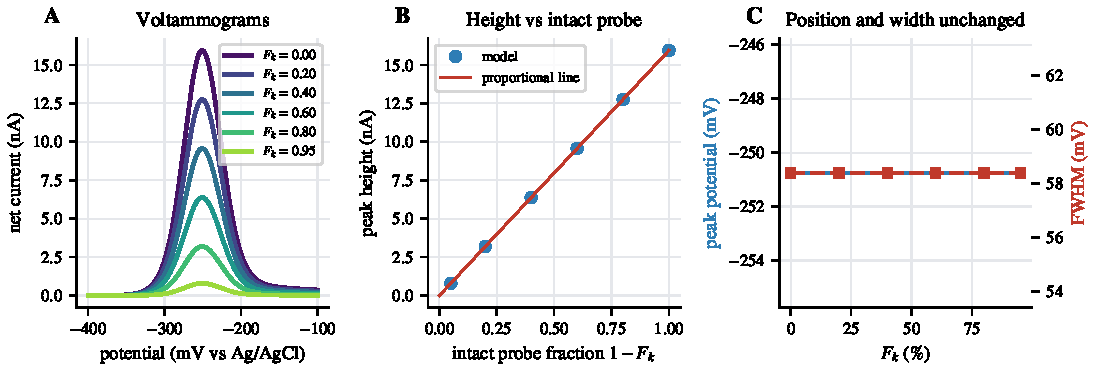
\includegraphics[width=\textwidth]{swvr_10_cleavage_response.pdf}
\caption{\textbf{A:} Predicted voltammograms as probes are cut. \textbf{B:} The peak height is directly proportional to the fraction of intact probes. \textbf{C:} The peak position and width do not change with the fraction of intact probes.}
\label{fig:proportional}
\end{figure}

Adding up the signal from every label on the electrode shows that the peak height is exactly proportional to the number of intact probes, while its position and shape do not change. Most of the signal comes from a narrow band of labels around $0.25\nm$ above the spacer tip. Evaluating the total signal for a fresh electrode at $10\,\mathrm{Hz}$ gives a peak of $15.9\,\mathrm{nA}$ at $-251\,\mathrm{mV}$.

%=======================================================================
\section{Reading Out How Many Probes Were Cut}
\label{sec:readout}

In Section~\ref{sec:whole} we showed that the height of the MB peak in the square-wave voltammogram, the maximum net current the electrode produces, is proportional to the number of intact probes. If a fraction $F_k$ of the probes has been cut, the peak shrinks to $(1 - F_k)$ of its original height:
\begin{equation}
\Delta I(T) = (1 - F_k)\,\Delta I(0),
\label{eq:deltait}
\end{equation}
where $\Delta I(0)$ is the peak height before incubation, when no probes have been cut, and $\Delta I(T)$ is the peak height after an incubation time $T$. We therefore scan each electrode twice, once before adding the wound fluid, and once after incubation. Dividing the second peak by the first gives the fraction of probes still intact:
\begin{equation}
\frac{\Delta I(T)}{\Delta I(0)} = 1 - F_k.
\label{eq:ratio}
\end{equation}
Rearranging gives the fraction that were cut:
\begin{equation}
F_k = 1 - \frac{\Delta I(T)}{\Delta I(0)}
\label{eq:fk_readout}
\end{equation}
For example, if the peak falls from $15.9\,\mathrm{nA}$ to $7.7\,\mathrm{nA}$, then
\begin{equation}
F_k = 1 - \frac{7.7}{15.9} = 0.52,
\label{eq:fk_example}
\end{equation}
so 52\% of the probes were cut.

%=======================================================================
\section{Calculating How Fast MMP-9 Cuts the Probes}
\label{sec:kinetics}

So far, the model links the fraction of probes cut, $F_k$, to the peak we measure. The last step is to link $F_k$ to the amount of MMP-9 in the wound fluid, by working out how quickly the enzyme cuts the probes.

MMP-9 cuts each probe in two stages. First, the enzyme (let us call it E) finds a probe (let us call it S) and binds to it, forming an enzyme-probe complex (ES). The complex can either fall apart again, releasing the intact probe, or the enzyme can cut the peptide. Once it has cut, the enzyme is released unchanged and is free to move on to another probe:
\begin{equation}
\text{E} + \text{S}\;\underset{k_{-1}}{\overset{k_1}{\rightleftharpoons}}\;\text{ES}\;\xrightarrow{\;\kcat\;}\;\text{E} + \text{cut probe}.
\label{eq:scheme}
\end{equation}
Here $k_1$ is the rate at which the enzyme binds a probe, $k_{-1}$ is the rate at which the complex falls apart, and $\kcat$ is the rate at which the bound enzyme cuts the probe. Together these define the Michaelis constant,
\begin{equation}
\Km = \frac{k_{-1} + \kcat}{k_1},
\label{eq:km}
\end{equation}
which measures how readily the enzyme binds its target; a small $\Km$ means the enzyme binds tightly. Because the enzyme is never used up, a small amount of MMP-9 can cut many probes over time. The more MMP-9 there is, the faster this happens.

\subsection{Calculating the rate of cutting}
Let $S_T$ be the number of probes still intact. Using the reaction scheme above, the rate at which probes are cut is
\begin{equation}
\frac{dS_T}{dt} = -\frac{\kcat[\text{E}]}{\Km + [\text{E}]}\,S_T \;\approx\; -\keff\MMP\,S_T.
\label{eq:dstdt}
\end{equation}
The minus sign shows that the number of intact probes is falling. The simplification on the right holds because the MMP-9 concentration in wound fluid, $[\text{E}]$, is far smaller than $\Km = 1.3\,\mathrm{mM}$~\cit{13}, so $\Km + [\text{E}]\approx \Km$. The cutting rate is then simply proportional to both the number of intact probes and the MMP-9 concentration.

For our peptide in solution, $\frac{\kcat}{\Km} = 67{,}500\,\mathrm{M^{-1}\,s^{-1}}$, with $\kcat = 86.4\,\mathrm{s^{-1}}$~\cit{13}. On the electrode, the enzyme must reach probes that are tethered and surrounded by other molecules, so it cuts them more slowly. We account for this with a surface efficiency of 0.20, giving an effective rate constant of
\begin{equation}
\keff = 0.20\times67{,}500 = 13{,}500\,\mathrm{M^{-1}\,s^{-1}}.
\label{eq:keff}
\end{equation}

\begin{itemize}
  \item The enzyme-probe complex, ES, forms and breaks apart very quickly, within about $\frac{1}{\kcat}\approx12\,\mathrm{ms}$. The probes, on the other hand, are used up over minutes. So the amount of ES quickly settles to a steady level and stays there while the probes are slowly cut. This is the \textbf{quasi-steady-state approximation}. At steady state, ES forms as fast as it is lost:
  \[ \underbrace{k_1[\text{E}][\text{S}]}_{\text{formed}} = \underbrace{(k_{-1} + \kcat)[\text{ES}]}_{\text{lost by falling apart or cutting}}. \]
  Dividing both sides by $k_1$, and using the definition $\Km = \frac{k_{-1} + \kcat}{k_1}$:
  \[ [\text{E}][\text{S}] = \Km[\text{ES}]. \]
  The intact probes $S_T$ are either free (S) or bound in a complex (ES), so $[\text{S}] = S_T - [\text{ES}]$. Substituting this in we get
  \[ [\text{E}]\big(S_T - [\text{ES}]\big) = \Km[\text{ES}]. \]
  Now we can solve this for $[\text{ES}]$. Expanding and collecting the $[\text{ES}]$ terms on one side gives
  \[ [\text{E}]S_T = [\text{ES}]\big(\Km + [\text{E}]\big), \]
  So,
  \[ [\text{ES}] = \frac{[\text{E}]}{\Km + [\text{E}]}\,S_T. \]
  \item Each complex cuts its probe at rate $\kcat$, and each cut removes one intact probe, so
  \[ \frac{dS_T}{dt} = -\kcat[\text{ES}] = -\frac{\kcat[\text{E}]}{\Km + [\text{E}]}\,S_T. \]
  \item A chronic wound has about 30 nM of MMP-9, while $\Km = 1.3\,\mathrm{mM}$. The ratio is
  \[ \frac{[\text{E}]}{\Km} = \frac{30\times10^{-9}}{1.3\times10^{-3}} = 2.3\times10^{-5}, \]
  which is tiny, so $\Km + [\text{E}]\approx \Km$ and
  \[ \frac{dS_T}{dt}\approx-\frac{\kcat}{\Km}\MMP\,S_T. \]
  \item The value $\frac{\kcat}{\Km} = 67{,}500\,\mathrm{M^{-1}\,s^{-1}}$ was measured for the peptide moving freely in solution~\cit{13}. On the electrode, each probe is tethered at one end and surrounded by other molecules, so MMP-9 cannot reach it as easily, and it is cut more slowly. We account for this with a surface efficiency $\eta = 0.20$, an estimate of how much more slowly MMP-9 cuts tethered probes. Plugging this in we get
  \[ \keff = \eta\,\frac{\kcat}{\Km} = 0.20\times67{,}500 = 13{,}500\,\mathrm{M^{-1}\,s^{-1}}, \]
  The rate equation then becomes
  \[ \frac{dS_T}{dt} = -\keff\MMP\,S_T. \]
  Multiplying $\keff$ by the MMP-9 concentration gives the chance per second that any one probe is cut. For a chronic wound (30 nM) this is about $4\times10^{-4}\,\mathrm{s^{-1}}$.
\end{itemize}

\subsection{Cut fraction over time}
The rate equation says that every intact probe has the same chance per second of being cut, so the number of intact probes falls exponentially with time. Solving it over an incubation time $T$ gives the fraction of probes that have been cut:
\begin{equation}
F_k(T) = 1 - e^{-\keff\MMP\,T}
\label{eq:fkt}
\end{equation}
At the start of the incubation ($T = 0$), no probes have been cut, so $F_k = 0$. As the incubation continues, $F_k$ rises towards 1 as nearly every probe is eventually cut. The higher the MMP-9 concentration, the faster this happens. This equation completes the model; it links the MMP-9 level in the wound to the fraction of probes cut, which in turn sets the peak height we measure.

\begin{itemize}
  \item From the previous step, the number of intact probes $S_T$ changes as
  \[ \frac{dS_T}{dt} = -\keff\MMP\,S_T. \]
  During the incubation, the MMP-9 concentration stays constant, since the enzyme is not used up. This means $\keff\MMP$ is just a constant.
  \item To solve this differential equation, we can divide both sides by $S_T$ and multiply by $dt$, so that everything involving $S_T$ is on one side and everything involving time is on the other:
  \[ \frac{dS_T}{S_T} = -\keff\MMP\,dt. \]
  \item Now we integrate both sides, from $t = 0$ (when there are $S_T(0)$ intact probes), to $t = T$ (when there are $S_T(T)$ intact probes):
  \[ \int_{S_T(0)}^{S_T(T)}\frac{dS_T}{S_T} = -\keff\MMP\int_0^T dt. \]
  The integral of $\frac{1}{S_T}$ is $\ln(S_T)$, so
  \[ \ln S_T(T) - \ln S_T(0) = -\keff\MMP\,T. \]
  \[ \ln\frac{S_T(T)}{S_T(0)} = -\keff\MMP\,T. \]
  Taking the exponential of both sides gives the fraction of probes still intact:
  \[ \frac{S_T(T)}{S_T(0)} = e^{-\keff\MMP\,T}. \]
  The fraction cut is one minus the fraction still intact, and is therefore
  \[ F_k(T) = 1 - e^{-\keff\MMP\,T}. \]
\end{itemize}

%=======================================================================
\section{Results}
\label{sec:results}

\subsection{Healing vs. chronic}
To see whether the sensor can tell the two wound types apart, we calculate the cut fraction after a 30-minute incubation for a healing wound (6 nM of MMP-9) and a chronic wound (30 nM):

\begin{table}[H]
\centering
\footnotesize\renewcommand{\arraystretch}{1.25}
\begin{tabular}{@{}lccc@{}}
\toprule
Wound & MMP-9 & Probes cut after 30 min & Peak after 30 min \\
\midrule
Healing & 6 nM & 14\% & 13.7 nA \\
Chronic & 30 nM & 52\% & 7.7 nA \\
\bottomrule
\end{tabular}
\caption{Predicted cut fraction and peak height after a 30-minute incubation, for a healing and a chronic wound.}
\label{tab:healing_chronic}
\end{table}

\begin{itemize}
  \item 30 minutes is $T = 30\times60 = 1800\,\mathrm{s}$, and the effective rate constant is $\keff = 13{,}500\,\mathrm{M^{-1}\,s^{-1}}$.
  \item \textbf{Chronic wound} ($30\,\mathrm{nM} = 30\times10^{-9}\,\mathrm{M}$) -- The exponent is
  \[ \keff\MMP\,T = 13{,}500\times30\times10^{-9}\times1800 = 0.729, \]
  \[ F_k = 1 - e^{-0.729} = 1 - 0.482 = 0.52 = 52\%. \]
  \item \textbf{Healing wound} ($6\,\mathrm{nM} = 6\times10^{-9}\,\mathrm{M}$) -- The exponent is
  \[ \keff\MMP\,T = 13{,}500\times6\times10^{-9}\times1800 = 0.146, \]
  \[ F_k = 1 - e^{-0.146} = 1 - 0.864 = 0.14 = 14\%. \]
  \item From Section~\ref{sec:readout}, the peak height after incubation is
  \[ \Delta I(T) = (1 - F_k)\,\Delta I(0), \]
  with $\Delta I(0) = 15.9\,\mathrm{nA}$ for a fresh electrode:
  \[ \text{Healing: } 0.864\times15.9 = 13.7\,\mathrm{nA}, \qquad \text{Chronic: } 0.482\times15.9 = 7.7\,\mathrm{nA}. \]
\end{itemize}

A chronic wound cuts over half of the probes in 30 minutes, while a healing wound cuts only about one in seven. This gives a large, easily measured difference in the peak, from 15.9 nA before incubation down to 13.7 nA for a healing wound, compared with 7.7 nA for a chronic one. So, the sensor can distinguish the two wound types within 30 minutes. Figure~\ref{fig:calibration} shows the model's predictions across a wider range of MMP-9 concentrations and incubation times.

\begin{figure}[H]
\centering
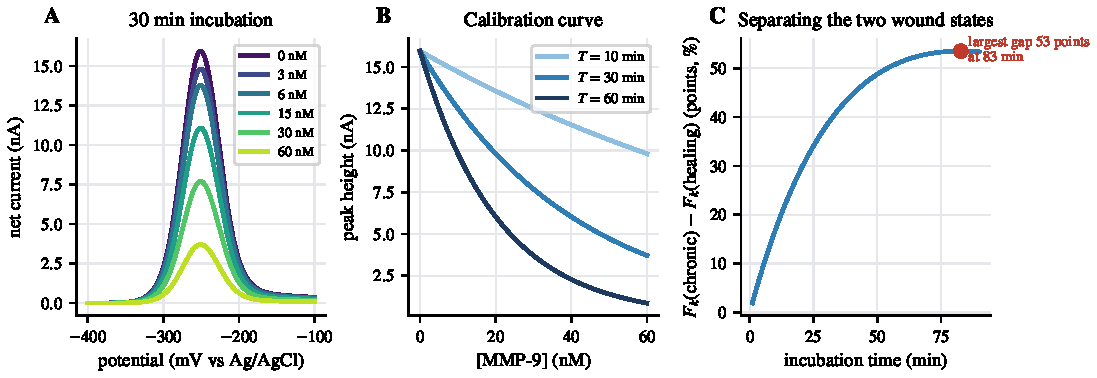
\includegraphics[width=\textwidth]{swvr_20_voltammograms.pdf}
\caption{The complete model. \textbf{A:} Predicted voltammograms after a 30-minute incubation for different MMP-9 concentrations. \textbf{B:} Predicted peak height against MMP-9 concentration for three incubation times. \textbf{C:} The difference in cut fraction between chronic and healing wounds grows with incubation time, peaking at 83 minutes.}
\label{fig:calibration}
\end{figure}

%=======================================================================
\section{Conclusion}
\label{sec:conclusion}

The model shows that the height of the MB peak is exactly proportional to the number of intact probes, so it falls in direct proportion to the fraction of probes MMP-9 has cut. Comparing each electrode before and after incubation therefore gives the cut fraction directly, and enzyme kinetics turns this into an MMP-9 concentration.

Applying the model to typical wound levels, a healing wound (6 nM) is predicted to cut about 14\% of the probes in 30 minutes, while a chronic wound (30 nM) cuts about 52\%. The corresponding peaks, 13.7 nA and 7.7 nA, are clearly different, showing that the sensor can separate healing from chronic wounds within 30 minutes.

%=======================================================================
\section*{Parameters}

\begin{table}[H]
\centering
\footnotesize\renewcommand{\arraystretch}{1.25}
\begin{tabular}{@{}llll@{}}
\toprule
Symbol & Meaning & Value & Source \\
\midrule
$\Gtot$ & Probe coverage & $3\,\mathrm{pmol\,cm^{-2}}$ & \cit{2} \\
$A$ & Electrode area & $0.017\,\mathrm{cm^2}$ & Our device \\
$b$ & Kuhn length of peptide & $0.76\,\mathrm{nm}$ & \cit{3} \\
$\dpeg$ & Height of spacer tip & $1.40\,\mathrm{nm}$ & Section~\ref{sec:label} \\
$\beta$ & Tunnelling decay constant & $10\,\mathrm{nm^{-1}}$ & \cit{4,5} \\
$\kref$ & Rate constant at spacer tip & $127\,\mathrm{s^{-1}}$ & \cit{6}, Section~\ref{sec:label} \\
$\alpha,\ n_e$ & Transfer coefficient, electrons & 0.37, 2 & \cit{6,10} \\
$E^0$ & Formal potential of MB & $-0.25\,\mathrm{V}$ vs Ag/AgCl & \cit{6} \\
$f$ & SWV frequency & $10\,\mathrm{Hz}$ & Our device \\
$E_{\mathrm{sw}}$ & Square-wave amplitude & $25\,\mathrm{mV}$ & Our device \\
$\Km$ & Michaelis constant & $1.3\,\mathrm{mM}$ & \cit{13} \\
$\kcat$ & MMP-9 turnover rate & $86.4\,\mathrm{s^{-1}}$ & \cit{13} \\
$\kcat/\Km$ & MMP-9 cutting rate (solution) & $67\,500\,\mathrm{M^{-1}s^{-1}}$ & \cit{13} \\
$\eta$ & Surface efficiency & 0.20 & Section~\ref{sec:kinetics} \\
$\keff$ & MMP-9 cutting rate (surface) & $13\,500\,\mathrm{M^{-1}s^{-1}}$ & Section~\ref{sec:kinetics} \\
\bottomrule
\end{tabular}
\caption{Model parameters, their values and sources.}
\label{tab:parameters}
\end{table}

%=======================================================================
\section*{References}

\begin{enumerate}[label={[\arabic*]},noitemsep,leftmargin=*]
\item Trengove NJ, Stacey MC, MacAuley S, Bennett N, Gibson J, Burslem F,
  Murphy G, Schultz G (1999). Analysis of the acute and chronic wound
  environments: the role of proteases and their inhibitors.
  \textit{Wound Repair Regen} 7:442--452.

\item Adj\'emian J, Anne A, Cauet G, Demaille C (2010). Cleavage-sensing
  redox peptide monolayers for the rapid measurement of the proteolytic
  activity of trypsin and $\alpha$-thrombin enzymes.
  \textit{Langmuir} 26:10347--10356.

\item Kohn JE, Millett IS, Jacob J, et al.\ (2004). Random-coil behavior
  and the dimensions of chemically unfolded proteins.
  \textit{PNAS} 101:12491--12496.

\item Smalley JF, Feldberg SW, Chidsey CED, Linford MR, Newton MD, Liu Y-P
  (1995). The kinetics of electron transfer through ferrocene-terminated
  alkanethiol monolayers on gold. \textit{J Phys Chem} 99:13141--13149.

\item Chidsey CED (1991). Free energy and temperature dependence of
  electron transfer at the metal-electrolyte interface.
  \textit{Science} 251:919--922.

\item Dauphin-Ducharme P, Arroyo-Curr\'as N, Kurnik M, Ortega G, Li H,
  Plaxco KW (2017). Simulation-based approach to determining electron
  transfer rates using square-wave voltammetry.
  \textit{Langmuir} 33(18):4407--4413.

\item Bard AJ, Faulkner LR (2001). Electrochemical Methods: Fundamentals
  and Applications, 2nd ed. Wiley.

\item Laviron E (1979). The use of linear potential sweep voltammetry and
  of a.c.\ voltammetry for the study of the surface electrochemical
  reaction of strongly adsorbed systems and of redox modified electrodes.
  \textit{J Electroanal Chem} 100:263--270.

\item Marcus RA (1965). On the theory of electron-transfer reactions.
  VI. Unified treatment for homogeneous and electrode reactions.
  \textit{J Chem Phys} 43:679--701.

\item Baker BR, Lai RY, Wood MS, Doctor EH, Heeger AJ, Plaxco KW (2006).
  An electronic, aptamer-based small-molecule sensor for the rapid,
  label-free detection of cocaine in adulterated samples and biological
  fluids. \textit{J Am Chem Soc} 128:3138--3139.

\item O'Dea JJ, Osteryoung J, Osteryoung RA (1981). Theory of square wave
  voltammetry for kinetic systems. \textit{Anal Chem} 53:695--701.

\item Osteryoung JG, Osteryoung RA (1985). Square wave voltammetry.
  \textit{Anal Chem} 57:101A--110A.

\item Kridel SJ, Chen E, Kotra LP, Howard EW, Mobashery S, Smith JW
  (2001). Substrate hydrolysis by matrix metalloproteinase-9.
  \textit{J Biol Chem} 276(23):20572--20578.
\end{enumerate}

\end{document}
